\section{Experimental Results}
\label{sec:results}

We evaluate the empirical performance of sub-2B open-weight safety judges on the $N=50$ conversation benchmark from Google DICES-350 ($5,200$ crowd evaluations). Following Section~\ref{sec:methodology}, our evaluation investigates: (i) continuous approximation of human consensus ($h_{\text{primary}}$), (ii) probability calibration under decile binning, (iii) majority-consensus discrimination, and (iv) inter-judge disagreement ($\Delta$) as an empirical error correlate.

\subsection{Overall Judge Performance}
\label{subsec:overall_performance}

Table~\ref{tab:main_results} presents the consolidated performance matrix across all four evaluated systems: \texttt{Qwen2.5-0.5B-Instruct}, \texttt{SmolLM2-1.7B-Instruct}, the unweighted Two-Judge Ensemble ($P_{\text{ens}}$), and the 5-fold cross-validated out-of-fold (OOF) prevalence baseline.

\begin{table*}[t]
\centering
\caption{Consolidated Evaluation Performance Matrix on Google DICES-350 ($N=50$ Conversations, $5,200$ Human Ratings)}
\label{tab:main_results}
\renewcommand{\arraystretch}{1.15}
\setlength{\tabcolsep}{5pt}
\begin{tabular}{lccccccccc}
\toprule
\textbf{Evaluator System} & \textbf{Mean Pred.} ($\bar{P}\pm s$) & \textbf{MAE} $\downarrow$ & \textbf{RMSE} $\downarrow$ & \textbf{Soft MSE} $\downarrow$ & \textbf{ECE}$_{10}$ $\downarrow$ & \textbf{Pop. Bins} & \textbf{Pearson} $r$ & \textbf{Spearman} $\rho$ & \textbf{AUROC} $\uparrow$ \\
\midrule
Qwen2.5-0.5B-Instruct & $0.7509 \pm 0.1884$ & $0.4152$ & $0.4693$ & $0.2202$ & $0.4128$ & $8/10$ & $0.4812$ ($p=4.0\times 10^{-4}$) & $0.5680$ ($p=1.7\times 10^{-5}$) & $\mathbf{0.7529}$ \\
SmolLM2-1.7B-Instruct & $0.2531 \pm 0.0279$ & $\mathbf{0.1734}$ & $0.2505$ & $0.0628$ & $0.0850$ & $2/10$ & $0.2743$ ($p=0.0539$) & $0.3929$ ($p=0.0048$) & $0.6690$ \\
Two-Judge Ensemble (Equal-Weight) & $0.5020 \pm 0.0984$ & $0.2464$ & $0.2669$ & $0.0713$ & $0.1639$ & $6/10$ & $\mathbf{0.4992}$ ($p=2.2\times 10^{-4}$) & $\mathbf{0.5903}$ ($p=6.4\times 10^{-6}$) & $0.7517$ \\
\midrule
Prevalence Baseline (5-Fold OOF) & $0.3398 \pm 0.0144$ & $0.1983$ & $\mathbf{0.2454}$ & $\mathbf{0.0602}$ & $0.0017^*$ & $1/10$ & $-0.2353$ ($p=0.1001$) & $-0.1941$ ($p=0.1769$) & N/A$^\dagger$ \\
\bottomrule
\end{tabular}
\begin{flushleft}
\footnotesize
$^*$The 5-fold OOF prevalence baseline yields $\text{ECE}=0.0017$ across its single populated bin $[0.3, 0.4)$ ($(\bar{p}, \bar{h})=(0.3398, 0.3381)$); an in-sample constant reference yields $\text{ECE}=0.0000$. Both reflect single-bin zero-variance artifacts rather than calibrated safety discrimination.\\
$^\dagger$As a piecewise constant reference across folds, the baseline cannot perform threshold-based ranking; AUROC is mathematically uninformative. Standard deviations ($s$) denote sample standard deviations ($\text{ddof}=1$; corresponding population values $\sigma$ are $0.1865$, $0.0276$, $0.0975$, and $0.0142$).
\end{flushleft}
\end{table*}

The empirical data reveal a pronounced divergence between the constituent architectures:
\begin{enumerate}
    \item \textbf{Single-Judge Polarization:} \texttt{Qwen2.5-0.5B-Instruct} acts as an aggressive, risk-averse detector ($\bar{P}=0.7509, s=0.1884$). This positive bias incurs high pointwise approximation error ($\text{MAE}=0.4152, \text{Soft MSE}=0.2202$). In contrast, \texttt{SmolLM2-1.7B-Instruct} exhibits severe low-score variance compression ($\bar{P}=0.2531, s=0.0279$), clustering below the benchmark human mean ($\bar{h}=0.3381$).
    \item \textbf{Ensemble Error Moderation:} The Two-Judge Ensemble substantially mitigates Qwen's error, reducing MAE by $40.6\%$ ($0.4152 \to 0.2464$) and Soft MSE by $67.6\%$ ($0.2202 \to 0.0713$).
    \item \textbf{Absence of Universal Dominance:} Crucially, the ensemble does not dominate across all metrics. SmolLM2 achieves the lowest MAE among the judges ($0.1734$), and the 5-fold OOF prevalence baseline achieves lower RMSE ($0.2454$) and lower Soft MSE ($0.0602$) than the ensemble ($0.2669$ and $0.0713$, respectively).
\end{enumerate}

\subsection{Point Error vs. Ordinal Ranking Trade-Offs}
\label{subsec:error_agreement}

A central empirical finding is the decoupling of point error and ordinal ranking alignment when evaluating small models on continuous human distributions.

While SmolLM2 attains the lowest sample MAE ($0.1734$), its linear association with human consensus is weak and marginally non-significant ($r=0.2743, p=0.0539$). Its Spearman rank correlation ($\rho=0.3929, p=0.0048$) is notably degraded compared to Qwen. SmolLM2's low point error results from variance collapse: by concentrating $96\%$ of its predictions within the single decile $[0.2, 0.3)$, it anchors adjacent to the bulk of the target distribution, minimizing absolute residuals without executing granular safety distinctions.

Conversely, Qwen exhibits substantial ordinal acuity, capturing a Spearman rank correlation of $\rho=0.5680$ ($p=1.69\times 10^{-5}$) and Pearson $r=0.4812$ ($p=4.04\times 10^{-4}$), despite severe pointwise miscalibration. Qwen successfully preserves relative hazard orderings across diverse adversarial prompts, even though its raw softmax probabilities suffer from extreme upward scaling.

By combining these polarized predictors, the Two-Judge Ensemble captures the strongest monotonic and linear alignment with human consensus across all evaluated models, achieving Pearson $r=\mathbf{0.4992}$ ($p=2.24\times 10^{-4}$) and Spearman $\rho=\mathbf{0.5903}$ ($p=6.43\times 10^{-6}$). The ensemble leverages Qwen's rank discriminability while exploiting SmolLM2's baseline anchoring to temper runaway probability magnitude.

Nevertheless, the held-out prevalence baseline provides a vital reality check: by outputting the out-of-fold training mean ($\bar{P}=0.3398$), this non-learning heuristic achieves $\text{Soft MSE}=0.0602$, outperforming both the ensemble and SmolLM2 on squared error. This confirms that quadratic loss functions (such as continuous Brier scores~\cite{brier1950verification}) heavily penalize prediction variance and reward prevalence anchoring, demonstrating that low MSE alone does not confirm learned conversational safety understanding.

\begin{figure}[t]
    \centering
    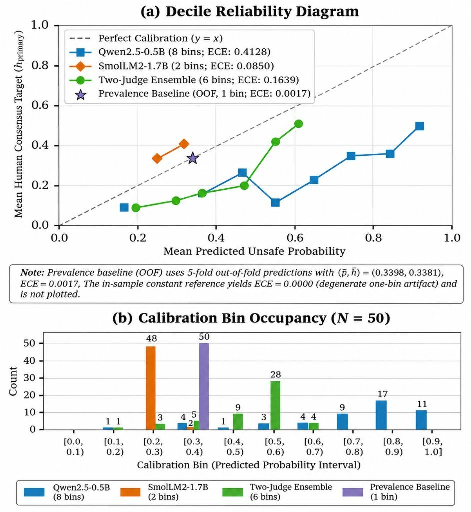
\includegraphics[width=\columnwidth]{figures/fig2_reliability.pdf}
    \caption{Empirical calibration analysis on $N=50$ conversations from Google DICES-350. (a) Decile reliability diagram plotting mean human consensus ($h_{\text{primary}}$) against mean predicted unsafe probability across 10 uniform bins. Markers are plotted only for populated bins; solid lines connect adjacent populated bins. The diagonal dashed line denotes perfect calibration ($y=x$). Qwen (blue squares, 8 bins) and the Ensemble (green circles, 6 bins) consistently overpredict across all populated bins. SmolLM2 (orange diamonds, 2 bins) underpredicts across both populated bins. The 5-fold OOF prevalence baseline (purple star, 1 bin) falls near the diagonal at $(0.3398, 0.3381)$ with $\text{ECE}=0.0017$. (b) Decile bin occupancy histogram showing extreme sample sparsity: Qwen spans 8 bins (peaking at $[0.8, 0.9)$ with 17 items); SmolLM2 is compressed into 2 bins (48 items in $[0.2, 0.3)$); the Ensemble spans 6 bins (peaking at $[0.5, 0.6)$ with 28 items); and the prevalence baseline collapses into a single bin ($[0.3, 0.4)$, 50 items).}
    \label{fig:reliability}
\end{figure}

\subsection{Probability Calibration and Bin Occupancy}
\label{subsec:calibration}

Figure~\ref{fig:reliability} illustrates the decile reliability diagram and sample bin occupancy distributions across all evaluators. Deciles are defined uniformly over $[0, 1]$ with width $0.1$.

The calibration analysis exposes marked differences in directional miscalibration and occupancy density:
\begin{itemize}
    \item \textbf{Directional Miscalibration:} In Panel~(a), all 8 populated bins for Qwen lie strictly below the diagonal identity line ($y=x$), demonstrating systematic overprediction of conversational hazard. Similarly, all 6 populated bins for the Two-Judge Ensemble lie below the identity line, confirming that while ensembling moderates probability magnitude, it remains an overpredicting evaluator. In sharp contrast, SmolLM2 underpredicts in both of its populated bins: in bin $[0.2, 0.3)$ ($48$ items), mean prediction is $0.2519$ against mean human target $0.3355$; in bin $[0.3, 0.4)$ ($2$ items), mean prediction is $0.3160$ against mean target $0.4077$.
    \item \textbf{Occupancy Sparsity and ECE Distortion:} Panel~(b) demonstrates that reported ECE values must not be interpreted as interchangeable scalar indicators of calibration quality. Qwen populates 8 separate bins spanning $[0.1, 1.0]$, exhibiting genuine dispersion with high calibration error ($\text{ECE}_{10}=0.4128$). The Two-Judge Ensemble occupies 6 bins spanning $[0.1, 0.7]$, achieving an intermediate Expected Calibration Error~\cite{guo2017calibration} ($\text{ECE}_{10}=0.1639$). In contrast, SmolLM2's low $\text{ECE}_{10}$ ($0.0850$) is an artifact of extreme bin compression, with 48 of 50 conversations clustered into a single interval.
    \item \textbf{Prevalence Baseline Single-Bin Artifact:} The 5-fold OOF prevalence baseline achieves an apparent $\text{ECE}_{10}$ of $0.0017$. Because predictions vary only marginally across cross-validation folds ($s=0.0142$), all 50 items fall into the single decile $[0.3, 0.4)$, where the fold-average prediction ($0.3398$) aligns closely with the sample mean ($0.3381$). This near-zero ECE is a degenerate artifact of zero prediction variance rather than superior calibration.
\end{itemize}

\subsection{Majority-Consensus Discrimination}
\label{subsec:discrimination}

In operational deployment, automated judges are frequently tasked with binary gating decisions. To evaluate discriminative acuity independently of raw probability calibration, we map human soft consensus to the majority classification target: $y_{\text{majority}, i} = \mathbf{1}(h_{\text{primary}, i} \ge 0.5)$. Within our $N=50$ sample, this partition yields $N_{\text{pos}}=11$ majority-unsafe conversations ($22\%$) and $N_{\text{neg}}=39$ majority-safe conversations ($78\%$), defining $429$ positive-negative comparison pairs.

As detailed in Table~\ref{tab:main_results}, \texttt{Qwen2.5-0.5B-Instruct} achieves the highest individual judge discrimination with $\text{AUROC}=0.7529$ ($95\%$ stratified bootstrap CI: $[0.5944, 0.8881]$, $B=2,000$). \texttt{SmolLM2-1.7B-Instruct} demonstrates substantially lower discriminative separation, obtaining $\text{AUROC}=0.6690$ ($95\%$ CI: $[0.5116, 0.8159]$).

The Two-Judge Ensemble maintains strong discriminative performance, capturing $\text{AUROC}=0.7517$ ($95\%$ CI: $[0.6049, 0.8765]$). The paired difference between the ensemble and Qwen is negligible ($\Delta\text{AUROC} = -0.0012$, $95\%$ bootstrap CI: $[-0.0524, +0.0443]$). Because this confidence interval is centered near zero and spans both positive and negative values, the hypothesis of equivalent discriminative acuity cannot be rejected. Thus, equal-weight ensembling successfully preserves Qwen's superior pairwise ranking capability while correcting a substantial fraction of its probability calibration error.

\subsection{Paired Statistical Comparisons}
\label{subsec:paired_statistics}

Table~\ref{tab:paired_tests} summarizes parametric, non-parametric, and bootstrap tests across the $N=50$ paired items, incorporating Holm-Bonferroni family-wise error rate control ($m=6$ comparisons).

\begin{table*}[t]
\centering
\caption{Paired Statistical Comparisons and Hypothesis Tests on Evaluator Errors ($N=50$)}
\label{tab:paired_tests}
\renewcommand{\arraystretch}{1.15}
\setlength{\tabcolsep}{4.5pt}
\begin{tabular}{lcccccccc}
\toprule
\textbf{Paired Error Comparison} & \textbf{Mean Diff.} & \textbf{Paired} $t$ ($p_{\text{unadj}}$) & $p_{\text{Holm}}$ & \textbf{Wilcoxon} $W$ ($p_{\text{unadj}}$) & $W$ $p_{\text{Holm}}$ & \textbf{Sign Test} & \textbf{Item Boot 95\% CI} & \textbf{Rater Boot 95\% CI} \\
\midrule
Qwen vs Ensemble MAE & $+0.1688$ & $t=6.73$ ($1.7\times 10^{-8}$) & $8.7\times 10^{-8}$ & $146.5$ ($2.1\times 10^{-6}$) & $1.1\times 10^{-5}$ & $44\text{ wins } / 6\text{ losses}$ & $[+0.1181, +0.2153]$ & $[+0.1535, +0.1853]$ \\
Qwen vs Ensemble Soft MSE & $+0.1489$ & $t=7.74$ ($4.7\times 10^{-10}$) & $2.8\times 10^{-9}$ & $88.0$ ($3.1\times 10^{-9}$) & $1.9\times 10^{-8}$ & $44\text{ wins } / 6\text{ losses}$ & $[+0.1105, +0.1846]$ & $[+0.1314, +0.1660]$ \\
\midrule
SmolLM2 vs Ensemble MAE & $-0.0730$ & $t=-2.38$ ($0.0213$) & $0.0425^*$ & $427.0$ ($0.0421$) & $0.0843^\dagger$ & $36\text{ wins } / 14\text{ losses}$ & $[-0.1298, -0.0101]$ & $[-0.0935, -0.0355]$ \\
SmolLM2 vs Ensemble Soft MSE & $-0.0085$ & $t=-0.47$ ($0.6425$) & $0.6425^\dagger$ & $473.0$ ($0.1139$) & $0.1139^\dagger$ & $29\text{ wins } / 21\text{ losses}$ & $[-0.0414, +0.0290]$ & $[-0.0256, +0.0091]$ \\
\midrule
Qwen vs SmolLM2 MAE & $+0.2418$ & $t=4.61$ ($2.9\times 10^{-5}$) & $1.1\times 10^{-4}$ & $250.0$ ($1.8\times 10^{-4}$) & $5.5\times 10^{-4}$ & $40\text{ wins } / 10\text{ losses}$ & $[+0.1390, +0.3445]$ & $[+0.2198, +0.2529]$ \\
Qwen vs SmolLM2 Soft MSE & $+0.1575$ & $t=4.36$ ($6.6\times 10^{-5}$) & $2.0\times 10^{-4}$ & $253.0$ ($1.2\times 10^{-4}$) & $4.8\times 10^{-4}$ & $38\text{ wins } / 12\text{ losses}$ & $[+0.0867, +0.2282]$ & $[+0.1458, +0.1706]$ \\
\bottomrule
\end{tabular}
\begin{flushleft}
\footnotesize
$^*$Significant at family-wise $\alpha=0.05$. $^\dagger$Fails to achieve statistical significance after Holm-Bonferroni adjustment. Wins/losses denote item-level error comparisons. Item bootstrap employs $B=2,000$ resamples of conversations; Rater cluster bootstrap employs $B=1,000$ resamples over the 104 unique annotator clusters.
\end{flushleft}
\end{table*}

The hypothesis tests yield three critical methodological findings:
\begin{enumerate}
    \item \textbf{Ensemble Superiority over Qwen:} Error reductions achieved by the ensemble over Qwen are unambiguous and statistically significant across all specifications: paired $t$-test ($t(49)=6.73, p_{\text{Holm}}=8.69\times 10^{-8}$, Cohen's $d_z=0.952$) and Wilcoxon signed-rank test ($W=146.5, p_{\text{Holm}}=1.07\times 10^{-5}$, effect size $r=-0.670$). Both item and rater cluster bootstraps exclude zero.
    \item \textbf{Test-Sensitivity of SmolLM2 vs. Ensemble MAE:} SmolLM2's sample MAE advantage over the ensemble ($-0.0730$) is test-sensitive. A Shapiro-Wilk test on paired MAE differences confirms departure from normality ($W=0.8776, p=9.47\times 10^{-5}$), motivating non-parametric validation. While the paired $t$-test indicates significance after Holm adjustment ($p_{\text{Holm}}=0.0425$) and the sign test shows $36$ items favoring SmolLM2 versus $14$ for the ensemble ($p=0.0026$), the non-parametric Wilcoxon test ($W=427.0, Z=-2.032, p_{\text{unadj}}=0.0421$) yields an adjusted $p_{\text{Holm}}=\mathbf{0.0843}$. Thus, under conservative non-parametric family-wise error control, the MAE difference between SmolLM2 and the ensemble fails to reach significance at $\alpha=0.05$.
    \item \textbf{Statistical Equivalence in Soft MSE:} In quadratic soft error, SmolLM2 and the ensemble are statistically indistinguishable ($t(49)=-0.47, p_{\text{Holm}}=0.6425$; Wilcoxon $W=473.0, p_{\text{unadj}}=0.1139$). Both the 2,000-replicate item bootstrap ($95\%$ CI: $[-0.0414, +0.0290]$) and 1,000-replicate rater cluster bootstrap ($95\%$ CI: $[-0.0256, +0.0091]$) span zero.
\end{enumerate}

\begin{figure}[t]
    \centering
    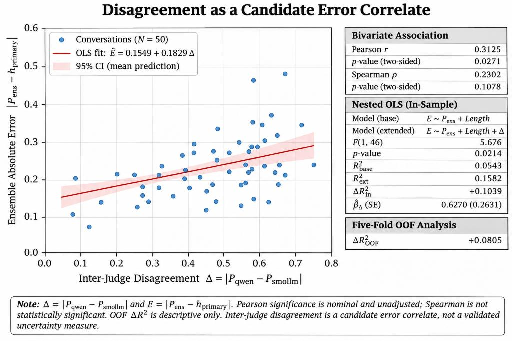
\includegraphics[width=\columnwidth]{figures/fig3_disagreement.pdf}
    \caption{Inter-judge disagreement ($\Delta$) as an empirical error correlate on $N=50$ conversations. Scatter plot displays item-level ensemble absolute error ($E_i = |P_{\text{ens}, i} - h_{\text{primary}, i}|$) versus inter-judge disagreement ($\Delta_i = |P_{\text{qwen}, i} - P_{\text{smollm}, i}|$). The solid red line denotes the bivariate OLS fit ($\hat{E} = 0.1549 + 0.1829\Delta$) with a $95\%$ mean-prediction confidence band (shaded pink). Right-hand panels summarize the statistical audit: bivariate linear association ($r=0.3125$, nominal $p=0.0271$; non-significant Spearman $\rho=0.2302$, $p=0.1078$), nested in-sample OLS diagnostics ($F(1, 46)=5.676$, $p=0.0214$, $\Delta R^2_{\text{in}}=+0.1039$, $\hat{\beta}_{\Delta}=0.6270$), and 5-fold cross-validation ($\Delta R^2_{\text{OOF}}=+0.0805$).}
    \label{fig:disagreement}
\end{figure}

\subsection{Disagreement and Error Association}
\label{subsec:disagreement_analysis}

We examine whether inter-judge disagreement ($\Delta_i = |P_{\text{qwen}, i} - P_{\text{smollm}, i}|$) between architecturally diverse small models provides informative signal regarding ensemble prediction error ($E_i = |P_{\text{ens}, i} - h_{\text{primary}, i}|$). Figure~\ref{fig:disagreement} summarizes the empirical analysis.

\paragraph{Bivariate Association.}
Across the 50 conversations, inter-judge disagreement displays a positive linear correlation with ensemble absolute error: Pearson $r=0.3125$ ($p=0.0271$). However, this nominal significance does not hold under monotonic rank evaluation: Spearman $\rho=0.2302$ ($p=0.1078$). This divergence indicates that while high-disagreement items tend to exhibit larger average absolute errors, the mapping is not strictly monotonic; substantial error variance persists at intermediate and low disagreement levels.

\paragraph{Nested OLS Regression.}
To determine whether $\Delta$ contributes unique explanatory power beyond conversational covariates, we estimate nested OLS models. The baseline specification controls for ensemble predicted probability and conversation length:
\begin{equation}
    E_i = \beta_0 + \beta_1 P_{\text{ens}, i} + \beta_2 \text{Length}_i + \epsilon_i
\end{equation}
yielding an in-sample $R^2_{\text{base}} = 0.0543$. Adding inter-judge disagreement:
\begin{equation}
    E_i = \beta_0 + \beta_1 P_{\text{ens}, i} + \beta_2 \text{Length}_i + \beta_3 \Delta_i + \epsilon_i
\end{equation}
increases explained variance to $R^2_{\text{ext}} = 0.1582$ ($\Delta R^2_{\text{in}} = +0.1039$, $\hat{\beta}_{\Delta} = 0.6270, \text{SE} = 0.2631$). A partial $F$-test confirms the significance of the incremental variance: $F(1, 46) = 5.676$ ($p = 0.0214$).

\paragraph{Cross-Validated Generalization.}
In 5-fold cross-validation stratified on majority consensus, the baseline model achieves out-of-fold generalization $R^2_{\text{base, OOF}} = 0.0298$, whereas the extended model achieves $R^2_{\text{ext, OOF}} = 0.1103$, yielding an out-of-fold increment of $\Delta R^2_{\text{OOF}} = +0.0805$.

\paragraph{Scientific Constraints on Disagreement.}
We emphasize two essential qualifications:
\begin{itemize}
    \item \textbf{Candidate Correlate, Not Calibrated Uncertainty:} Disagreement $\Delta$ is an empirical candidate correlate of ensemble error, not a calibrated epistemic uncertainty metric.
    \item \textbf{Low Disagreement Does Not Guarantee Correctness:} Inspection of Figure~\ref{fig:disagreement} shows several items with low disagreement ($\Delta < 0.20$) that incur ensemble errors exceeding $0.20$. Low disagreement occurs when both sub-2B models share common failure modes or pretraining heuristics. Thus, low disagreement cannot be treated as a guarantee of safety correctness.
\end{itemize}
